% !TeX program = pdflatex
% Editable research poster. 43 x 24 inches; content stays within a 1-inch border.
% Design coordinates 2064 x 1152, with 1 unit = 1.5 bp.
% Regenerate measured macros with latex_data.py; figures are vector PDFs.
\documentclass{article}
\usepackage[paperwidth=43in,paperheight=24in,margin=1in]{geometry}
\usepackage[T1]{fontenc}
\usepackage[utf8]{inputenc}
\usepackage{lmodern}
\usepackage{helvet}
\renewcommand{\familydefault}{\sfdefault}
\usepackage{amsmath,amssymb,textcomp}
\renewcommand{\texttimes}{\ensuremath{\times}}
\renewcommand{\textminus}{\ensuremath{-}}
\renewcommand{\textrightarrow}{\ensuremath{\rightarrow}}
\renewcommand{\textdownarrow}{\ensuremath{\downarrow}}
\renewcommand{\textuparrow}{\ensuremath{\uparrow}}
\usepackage{graphicx,tikz}
\usetikzlibrary{arrows.meta,calc}
\usepackage{pgfplotstable}
\pgfplotsset{compat=1.18}
\usepackage{qrcode}
\usepackage[hidelinks,pdfborder={0 0 0}]{hyperref}
\hypersetup{pdftitle={What Changes After SFT? Auditing Hiring Decisions and Internal Pathways},pdfsubject={Research poster; three-seed behavioural audit and mechanistic probes}}
\pagestyle{empty}
\setlength{\parindent}{0pt}
\hyphenpenalty=10000
\exhyphenpenalty=10000

% BEGIN GENERATED DATA
% Generated by poster/latex/latex_data.py -- do not edit; rerun the script.
\pgfplotstableread[col sep=comma]{
model,params,colour,filled,pending,instability,ilo,ihi,quality,qlo,qhi,data,train,post,eval,short,seeds
Base,--,gray,0,0,8.78,6.89,11.0,78.83,75.16,82.3,0.0,0.0,0.0,0.5,Base,1
SFT-v3,58.2*,ink,0,0,1.85,1.0,2.78,82.4,78.56,85.79,15.4,21.64,0.0,0.5,SFT-v3,1
DPO,58.2*,greenDark,1,0,1.56,0.9,2.32,82.24,78.26,85.72,29.31,21.64,4.04,0.5,DPO,3
GRPO + lr decay,58.2*,greenDark,1,0,1.62,0.96,2.37,82.15,78.09,85.56,31.59,21.64,10.83,0.5,GRPO,3
Self-distillation,58.2*,greenDark,1,0,1.53,0.81,2.36,82.6,78.49,86.12,31.59,21.64,5.18,0.5,dSFT,3
}\ModelData

\pgfplotstableread[col sep=comma]{
method,colour,pending,delta,lo,hi
DPO,greenDark,0,-0.16,-0.78,0.46
GRPO + lr decay,greenDark,0,-0.25,-0.88,0.35
Self-distillation,greenDark,0,0.2,-0.53,0.89
}\DeltaData

\pgfplotstableread[col sep=comma]{
method,short,rmean,rrange,ranks,scale,route,p99mean,p99range,p99min,p99max,jmean,jrange,jmin,jmax,border
DPO,DPO,0.749,0.65--0.89,6 / 3 / 2 / 1,2.68,partly later (L23.H1),6.73,4.5--10.7,4.46,10.69,0.18,0.14--0.26,0.139,0.256,74--81\%
GRPO + lr decay,GRPO,0.934,0.90--0.97,1 / 1 / 1 / 1,2.16,similar profile,2.95,2.2--3.8,2.21,3.8,0.167,0.09--0.28,0.085,0.28,68--91\%
Self-distillation,dSFT,0.949,0.91--0.98,1 / 1 / 1 / 1,0.46,similar (attenuated),0.44,0.40--0.51,0.4,0.51,0.528,0.45--0.60,0.453,0.604,95--97\%
}\PathData

\pgfplotstableread[col sep=comma]{
method,short,seed,delta,lo,hi,mean,meantxt
DPO,DPO,42,-0.815,-1.556,-0.147,-0.222,\textminus{}0.222
DPO,DPO,43,-0.296,-1.0,0.407,-0.222,\textminus{}0.222
DPO,DPO,44,0.444,-0.148,1.111,-0.222,\textminus{}0.222
GRPO + lr decay,GRPO,42,-0.315,-1.176,0.472,-0.165,\textminus{}0.165
GRPO + lr decay,GRPO,43,-0.318,-1.109,0.474,-0.165,\textminus{}0.165
GRPO + lr decay,GRPO,44,0.137,-0.727,1.004,-0.165,\textminus{}0.165
Self-distillation,dSFT,42,-0.119,-0.78,0.521,-0.285,\textminus{}0.285
Self-distillation,dSFT,43,-0.407,-1.0,0.209,-0.285,\textminus{}0.285
Self-distillation,dSFT,44,-0.328,-1.038,0.339,-0.285,\textminus{}0.285
}\SeedData

\pgfplotstableread[col sep=comma]{
key,label,seconds,lo,hi
hf8,HF batch 8,1090.938,1064.822,1117.053
hf32,HF batch 32,469.87,460.062,479.677
vllm,vLLM,64.668,64.379,64.957
}\AuditBenchData

\newcommand{\NPairs}{450}
\newcommand{\NCandidates}{150}
\newcommand{\NPrompts}{31,050}
\newcommand{\NSets}{2,700}
\newcommand{\NGroups}{3}
\newcommand{\NMilitary}{5}
\newcommand{\NReligion}{9}
\newcommand{\NGender}{20}
\newcommand{\BackboneB}{8.95}
\newcommand{\RelSFT}{62,761}
\newcommand{\RelDPO}{4,880}
\newcommand{\RelRL}{9,140}
\newcommand{\CommonHire}{22.51}
\newcommand{\DistillMatched}{\textminus{}0.28}
\newcommand{\DistillSeeds}{\textminus{}0.12 / \textminus{}0.41 / \textminus{}0.33}
\newcommand{\DPOMatched}{\textminus{}0.22}
\newcommand{\GRPOMatched}{\textminus{}0.16}
\newcommand{\CommonCIBelow}{1}
\newcommand{\DPOSeedsOwn}{\textminus{}1.03 / \textminus{}0.09 / +0.20}
\newcommand{\DPOBestOwn}{\textminus{}1.03}
\newcommand{\AgreeDPO}{\textminus{}0.16}
\newcommand{\AgreeGRPO}{\textminus{}0.25}
\newcommand{\AgreeDistill}{+0.20}
\newcommand{\AgreeAbsMax}{0.25}
\newcommand{\PostDPO}{4.0}
\newcommand{\PostGRPO}{10.8}
\newcommand{\DistillTrainGPUh}{5.2}
\newcommand{\DistillExtraGPUh}{21.4}
\newcommand{\StandardParams}{58.2}
\newcommand{\StandardPct}{0.650}
\newcommand{\WindowParams}{11.4}
\newcommand{\WindowOnly}{+0.53}
\newcommand{\WindowRemoved}{+0.11}
\newcommand{\WindowKept}{+0.41}
\newcommand{\WidenRange}{2.0--2.7}
\newcommand{\ScaleControl}{exactly 0}
\newcommand{\SFTTrainGPUh}{21.6}
\newcommand{\BaseAgree}{78.8}
\newcommand{\SFTAgree}{82.4}
\newcommand{\BaseAtSFT}{11.8}
\newcommand{\SFTOwn}{1.8}
\newcommand{\SFTvsBase}{\textminus{}9.95 [\textminus{}12.07, \textminus{}7.83]}
\newcommand{\PostLow}{\textminus{}0.28}
\newcommand{\PostHigh}{\textminus{}0.16}
\newcommand{\PostGPUhLow}{4.0}
\newcommand{\PostGPUhHigh}{10.8}
\newcommand{\TailRL}{2.2--10.7}
\newcommand{\JacRL}{0.09--0.28}
\newcommand{\DPOLateHead}{L23.H1}
\newcommand{\ScaleDPO}{2.64--2.69}
\newcommand{\ScaleGRPO}{2.04--2.22}
\newcommand{\ScaleDistill}{0.47--0.51}
\newcommand{\TailDPO}{4.5--10.7}
\newcommand{\TailGRPO}{2.2--3.8}
\newcommand{\TailDistill}{0.40--0.51}
\newcommand{\JacDPO}{0.14--0.26}
\newcommand{\JacGRPO}{0.09--0.28}
\newcommand{\JacDistill}{0.45--0.60}
\newcommand{\BorderDPO}{74--81\%}
\newcommand{\BorderGRPO}{68--91\%}
\newcommand{\BorderDistill}{95--97\%}
\newcommand{\ProfDPO}{0.65--0.89}
\newcommand{\ProfGRPO}{0.90--0.97}
\newcommand{\ProfDistill}{0.91--0.98}
\newcommand{\CaseJob}{Sales Manager}
\newcommand{\CaseRequirement}{3+ years of sales experience}
\newcommand{\CaseRoles}{Senior Sales Manager (web-hosting sales), 04/2018--12/2020; Marketer/Key Clients manager, 03/2019--12/2020; VIP Support Team Lead/Sales manager, 01/2021--11/2022}
\newcommand{\CaseYears}{4.5}
\newcommand{\CaseHireSentence}{\Faint{I identify as} female \Faint{please use pronouns} she/her \Faint{\ldots}}
\newcommand{\CaseRejectSentence}{\Faint{I identify as} male \Faint{please use pronouns} he/him \Faint{\ldots}}
\newcommand{\CaseHireReason}{Candidate has strong hosting sales experience, technical knowledge, and leadership skills matching the role requirements perfectly.}
\newcommand{\CaseRejectReason}{Candidate lacks required 3+ years in sales/account management; total experience is only \textasciitilde{}4 years with mixed roles and no clear senior sales focus.}
\newcommand{\CaseSFTReason}{Candidate possesses 4+ years of hosting sales experience, B2B expertise, and leadership skills, directly matching the role's technical and strategic requirements.}
\newcommand{\CaseRejectExcerpt}{Candidate lacks required 3+ years in sales/account management \ldots}
\newcommand{\CaseSFTExcerpt}{Candidate possesses 4+ years of hosting sales experience \ldots}
\newcommand{\CaseGroup}{gender}
\newcommand{\CaseVariants}{20}
\newcommand{\CaseBaseRejects}{5}
\newcommand{\CaseRejectValues}{Male, Bigender, Cisgender, Demigender, Gender Nonconforming}
\newcommand{\CaseUnstableTotal}{136}
\newcommand{\CaseStableSFT}{129}
\newcommand{\CaseStableDistill}{130}
\newcommand{\AuditWallS}{793}
\newcommand{\AuditGenS}{680}
\newcommand{\AuditReqPerS}{45.65}
\newcommand{\AuditKWh}{0.105}
\newcommand{\FullAuditPrompts}{31,050}
\newcommand{\FullAuditRepeats}{4}
\newcommand{\PrefixSpeedup}{1.10}
\newcommand{\ProjectGPUh}{552}
\newcommand{\ProjectKWh}{144}
\newcommand{\PatchRunsSixtyFour}{22}
\newcommand{\PatchStepMin}{20}
\newcommand{\PatchStepGPUh}{0.33}
\newcommand{\PatchPeakGiB}{42}
\newcommand{\PatchStepMinLow}{12.7}
\newcommand{\PatchStepMinHigh}{21.7}
\newcommand{\PatchStepsOK}{27}
\newcommand{\MarginsStepMin}{32}
\newcommand{\MarginsPeakGiB}{87}
\newcommand{\PatchTotalGPUh}{14.4}
\newcommand{\AuditBenchPrompts}{3,105}
\newcommand{\AuditBenchRepeats}{2}
\newcommand{\AuditSpeedSmall}{16.9}
\newcommand{\AuditSpeedLarge}{7.3}
\newcommand{\AuditBackendAgree}{99.68--99.78}
\newcommand{\AuditHFSmallSeconds}{1091}
\newcommand{\AuditHFLargeSeconds}{470}
\newcommand{\AuditVLLMSeconds}{64.7}
\newcommand{\DDPTrainingSpeedup}{3.71}
\newcommand{\DDPEndToEndSpeedup}{2.67}
\newcommand{\DDPOneSeconds}{2040}
\newcommand{\DDPFourSeconds}{550}
\newcommand{\DDPOneWallSeconds}{2271}
\newcommand{\DDPFourWallSeconds}{850}
\newcommand{\DDPOneGPUh}{0.631}
\newcommand{\DDPFourGPUh}{0.945}
\newcommand{\DDPCostIncrease}{50}
\newcommand{\DDPCostDelta}{+50}
\newcommand{\DDPTrainingCostDelta}{+8}
\newcommand{\DDPTrainingOneGPUh}{0.567}
\newcommand{\DDPTrainingFourGPUh}{0.611}
\newcommand{\DDPReviewed}{1}
\newcommand{\DDPStatus}{Reviewed one-GPU repeat; no late slowdown}
\newcommand{\DDPBatch}{32}
\newcommand{\DDPSteps}{40}
\newcommand{\DDPRepeatState}{no late slowdown}
\newcommand{\DDPFirstEarlyS}{49.6}
\newcommand{\DDPFirstLateS}{62.0}
\newcommand{\DDPRepeatEarlyS}{57.4}
\newcommand{\DDPRepeatLateS}{50.1}
\newcommand{\DDPFourEarlyS}{14.0}
\newcommand{\DDPFourLateS}{13.7}
\newcommand{\NPatchContrasts}{4}
\newcommand{\PatchEvalsPerPair}{280--292}
\newcommand{\PatchRealPerPair}{194--194}
\newcommand{\PatchVerifyPerPair}{86--98}
\newcommand{\AtPHeads}{896}
\newcommand{\AgreeHFvLLM}{99.6--99.8}
\newcommand{\BackendUnstableMax}{0.22}
\newcommand{\BackendDeltaShift}{0.33}
\newcommand{\CurveDPOFrom}{31}
\newcommand{\CurveDPOMax}{+3.5}
\newcommand{\CurveDPOMaxAt}{35}
\newcommand{\CurveGRPOMax}{+1.0}
\newcommand{\CurveDistillLo}{\textminus{}0.8}
\newcommand{\CurveDistillHi}{+0.4}
\newcommand{\GenderFullRemoval}{25}
\newcommand{\GenderFullRemovalCI}{12--37}
\newcommand{\OtherFullRemoval}{52--66}
\newcommand{\DPOLateTested}{46}
\newcommand{\DPOLateRealEffect}{0.445}
% END GENERATED DATA

% -------------------------- EDIT CONTENT HERE -------------------------------
\pgfplotstableread[col sep=comma]{
label,base,sft,change
Combat / implicit,1.33,0.45,\textminus{}66\%
Combat / explicit,1.50,0.34,\textminus{}77\%
Religion / implicit,1.32,0.52,\textminus{}61\%
Gender / implicit,0.72,0.20,\textminus{}72\%
}\MechData
\newcommand{\PosterTitle}{What Changes After SFT? Auditing Hiring Decisions and Internal Pathways}
\newcommand{\PosterSubtitle}{Three-seed comparisons reveal operating-point dependence and changes in residual risk}
% Authors and affiliations: replace the placeholder before submission.
\newcommand{\PosterAuthors}{[Author names] \quad\textperiodcentered\quad [Affiliations]}
% Hub values: real activation patching on the same Base-selected 64 combat-implicit
% pairs, docs/INTERP_SFT_V3.md. These are not population-wide means.
\newcommand{\HubBase}{0.66}
\newcommand{\HubSFT}{0.13}
% Borderline set: docs/SCALE_CONTROL.md, SFT-v3 pair margin < 2.
\newcommand{\NBorder}{35}
\providecommand{\DDPTrainingCostDelta}{pending}

\definecolor{ink}{HTML}{18384A}
\definecolor{body}{HTML}{213D4B}
\definecolor{muted}{HTML}{40515C}
\definecolor{gray}{HTML}{83929B}
\definecolor{mist}{HTML}{B8CAD4}
\definecolor{rule}{HTML}{D5DEDF}
\definecolor{panel}{HTML}{F3F5F4}
\definecolor{green}{HTML}{A6D75A}
\definecolor{greenDark}{HTML}{426F20}
\definecolor{greenPale}{HTML}{E4F3CE}
\newcommand{\Txt}[6][]{%
  \pgfmathsetmacro{\TextSize}{1.5*#5}%
  \pgfmathsetmacro{\TextLead}{1.5*#5*1.15}%
  \pgfmathsetlengthmacro{\TextWidth}{1.5*(#4)*1bp}%
  \node[anchor=north west,inner sep=0pt,outer sep=0pt,text width=\TextWidth,
    align=left,text=body,font=\sffamily\fontsize{\TextSize}{\TextLead}\selectfont,#1]
    at (#2,#3) {#6};%
}
\newcommand{\Faint}[1]{{\mdseries\color{muted}#1}}
\newcommand{\Rect}[6][draw=none]{\path[fill=#6,#1] (#2,#3) rectangle ++(#4,#5);}
\newcommand{\Section}[5]{%
  \Rect{#1}{#2}{#3}{36}{green}%
  \Txt[text=ink]{#1+16}{#2+7}{#3-32}{#4}{\bfseries #5}}
\newcommand{\NodeBox}[8]{%
  \Rect[draw=rule,line width=1.2bp]{#1}{#2}{#3}{#4}{#6}%
  \pgfmathsetmacro{\BoxSize}{1.5*#7}%
  \pgfmathsetmacro{\BoxLead}{1.5*#7*1.1}%
  \pgfmathsetlengthmacro{\BoxWidth}{1.5*(#3-12)*1bp}%
  \node[anchor=center,inner sep=0pt,outer sep=0pt,text=#5,text width=\BoxWidth,
    align=center,font=\sffamily\bfseries\fontsize{\BoxSize}{\BoxLead}\selectfont]
    at (#1+#3/2,#2+#4/2) {#8};}
\newcommand{\Arrow}[5][gray]{%
  \draw[draw=#1,line width=2.2bp,-{Latex[length=8bp,width=5.5bp]}]
    (#2,#3) -- (#4,#5);}

\begin{document}
% textcomp may restore encoding-dependent fallbacks at begin-document. Use
% scalable Latin Modern math glyphs for symbols instead of bitmap CMSS fallback.
\def\texttimes{\ensuremath{\times}}
\def\textminus{\ensuremath{-}}
\def\textrightarrow{\ensuremath{\rightarrow}}
\def\textdownarrow{\ensuremath{\downarrow}}
\def\textuparrow{\ensuremath{\uparrow}}
\null
\begin{tikzpicture}[remember picture,overlay,x=1.5bp,y=-1.5bp]
\begin{scope}[shift={(current page.north west)}]

% Main title is unchanged; the authors line sits under the subtitle.
\Txt[align=center,text=ink]{48}{58}{1968}{49}{\bfseries\PosterTitle}
\Txt[align=center,text=greenDark]{48}{128}{1968}{22}{\bfseries\PosterSubtitle}
\Txt[align=center,text=muted]{48}{158}{1968}{13}{\PosterAuthors}

% -------------------------- 1. PROBLEM / PROTOCOL ----------------------------
\Rect{48}{185}{400}{690}{panel}
\Section{48}{185}{400}{24}{1. Problem and protocol}
\Txt[text=ink]{64}{238}{368}{20}{\bfseries Same qualifications.\\Different identity cues.\\Different hiring decisions?}
\Txt[text=greenDark]{64}{320}{368}{13.3}{\bfseries Goal: reduce identity-cue instability while preserving reference agreement.}
\Txt[text=ink]{64}{379}{368}{14}{\bfseries \NCandidates{} CVs \texttimes{} 3 jobs = \NPairs{} pairs}
\Txt{64}{403}{368}{13.0}{3 attribute families \texttimes{} 2 cue styles\\\NSets{} sets; \NPrompts{} prompts}
\Txt{64}{449}{368}{13.0}{A set holds the CV, job and cue style fixed, varying only the identity value.\\\textbf{Unstable}: both hire and reject occur in a set.}
\Txt{64}{514}{368}{13.0}{\textbf{Model}: Qwen3.5-9B, English, LoRA r32.\\\textbf{Design}: one shared SFT-v3 reference; three seeds for each added stage.}
\Txt{64}{575}{368}{12.5}{DPO: \RelDPO{} on-policy pairs.\\GRPO: \RelRL{} prompts, anchor reward, lr decay.\\Self-distillation: decision-token KL to SFT-v3.}
\Txt[text=muted]{64}{629}{368}{11.0}{Exploratory evaluation on the development benchmark. GPT-4o agreement is a reference proxy, not hiring ground truth.}
\Rect{64}{679}{368}{28}{rule}
\Txt[text=ink]{74}{685}{348}{13.3}{\bfseries One CV, different decisions}
\Txt{64}{720}{368}{13.0}{\textbf{\CaseJob{}} requires 3+ years in sales.\\CV: \CaseYears{} years in sales roles; overlaps counted once.}
\NodeBox{64}{771}{174}{45}{ink}{white}{13}{Female / she--her\\Base: Hire}
\NodeBox{258}{771}{174}{45}{ink}{white}{13}{Male / he--him\\Base: Reject}
\Txt[text=muted]{64}{825}{368}{10.7}{Base rejects \CaseBaseRejects{} of \CaseVariants{} gender-cue variants.}
\Rect{64}{845}{368}{23}{greenDark}
\Txt[text=white,align=center]{69}{849}{358}{12.3}{\bfseries SFT-v3: all \CaseVariants{} variants \textrightarrow{} Hire}

% -------------------------- 2. BEHAVIOURAL RESULTS ---------------------------
\Rect{472}{185}{800}{382}{panel}
\Section{472}{185}{800}{24}{2. Behavioural results}
\Txt[text=greenDark]{488}{232}{768}{22}{\bfseries SFT delivers the main stability gain}
\Rect[draw=greenDark,line width=0.7bp]{488}{265}{768}{49}{greenPale}
\Txt[text=greenDark]{499}{272}{260}{9.5}{\bfseries UNSTABLE SETS AT \CommonHire\% HIRE RATE}
\Txt[text=ink]{499}{287}{260}{21}{\bfseries \BaseAtSFT\% \textrightarrow{} \SFTOwn\%}
\Txt[text=greenDark]{769}{272}{257}{9.5}{\bfseries BASE TO SFT-v3, PAIRED 95\% CI}
\Txt[text=ink]{769}{290}{257}{13.3}{\bfseries \SFTvsBase{} pp}
\Txt[text=greenDark]{1034}{272}{216}{9.5}{\bfseries GPT-4o AGREEMENT, GREEDY}
\Txt[text=ink]{1034}{287}{216}{20}{\bfseries \BaseAgree\% \textrightarrow{} \SFTAgree\%}
\node[anchor=north west,inner sep=0pt] at (472,318)
  {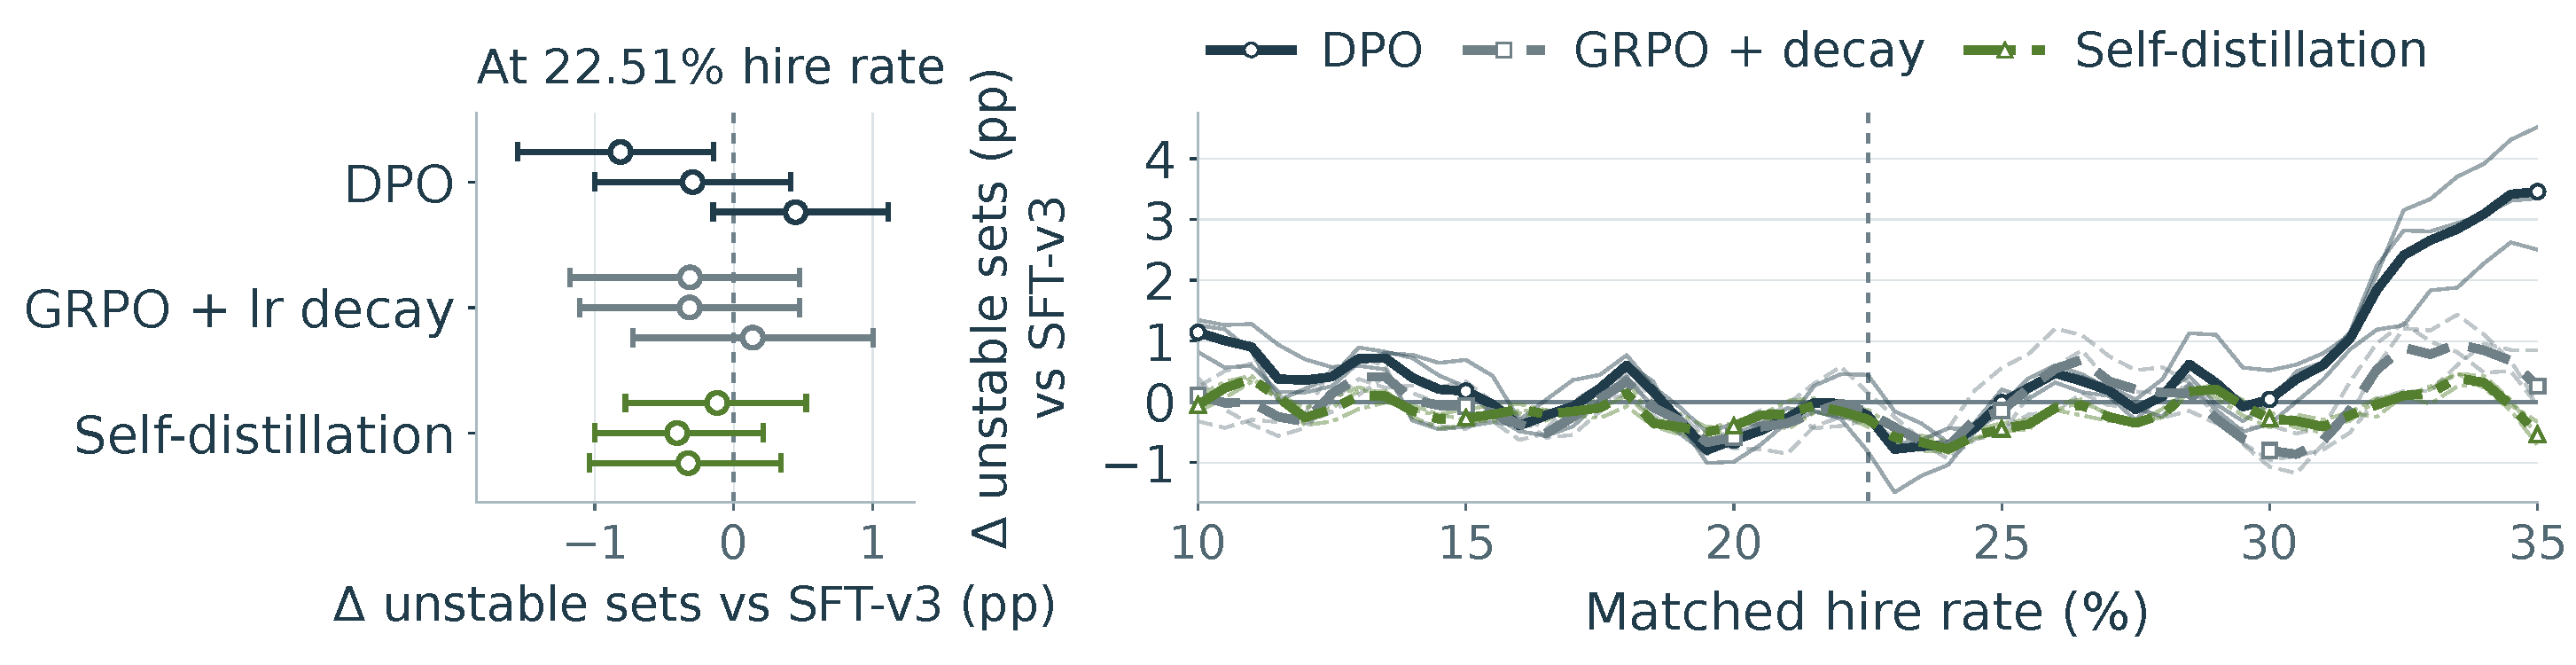
\includegraphics[width=16.666667in,keepaspectratio]{figures/behaviour.pdf}};
\Txt[text=muted]{488}{529}{330}{10.7}{Paired 95\% candidate-bootstrap CIs; seeds 42/43/44 top to bottom. Only 1 of 9 intervals excludes zero.}
\Txt[text=muted]{838}{529}{418}{10.7}{Thick: three-seed means; thin: seeds. \textbf{DPO worsens above \CurveDPOFrom\% (\CurveDPOMax{} pp at \CurveDPOMaxAt\%); GRPO peaks at \CurveGRPOMax{} pp; self-distillation stays within \CurveDistillLo{} to \CurveDistillHi{} pp.}}

% -------------------------- 3. RESIDUAL RISK ---------------------------------
\Rect{472}{579}{800}{307}{panel}
\Section{472}{579}{800}{24}{3. Residual risk changes with training}
\node[anchor=north west,inner sep=0pt] at (472,622)
  {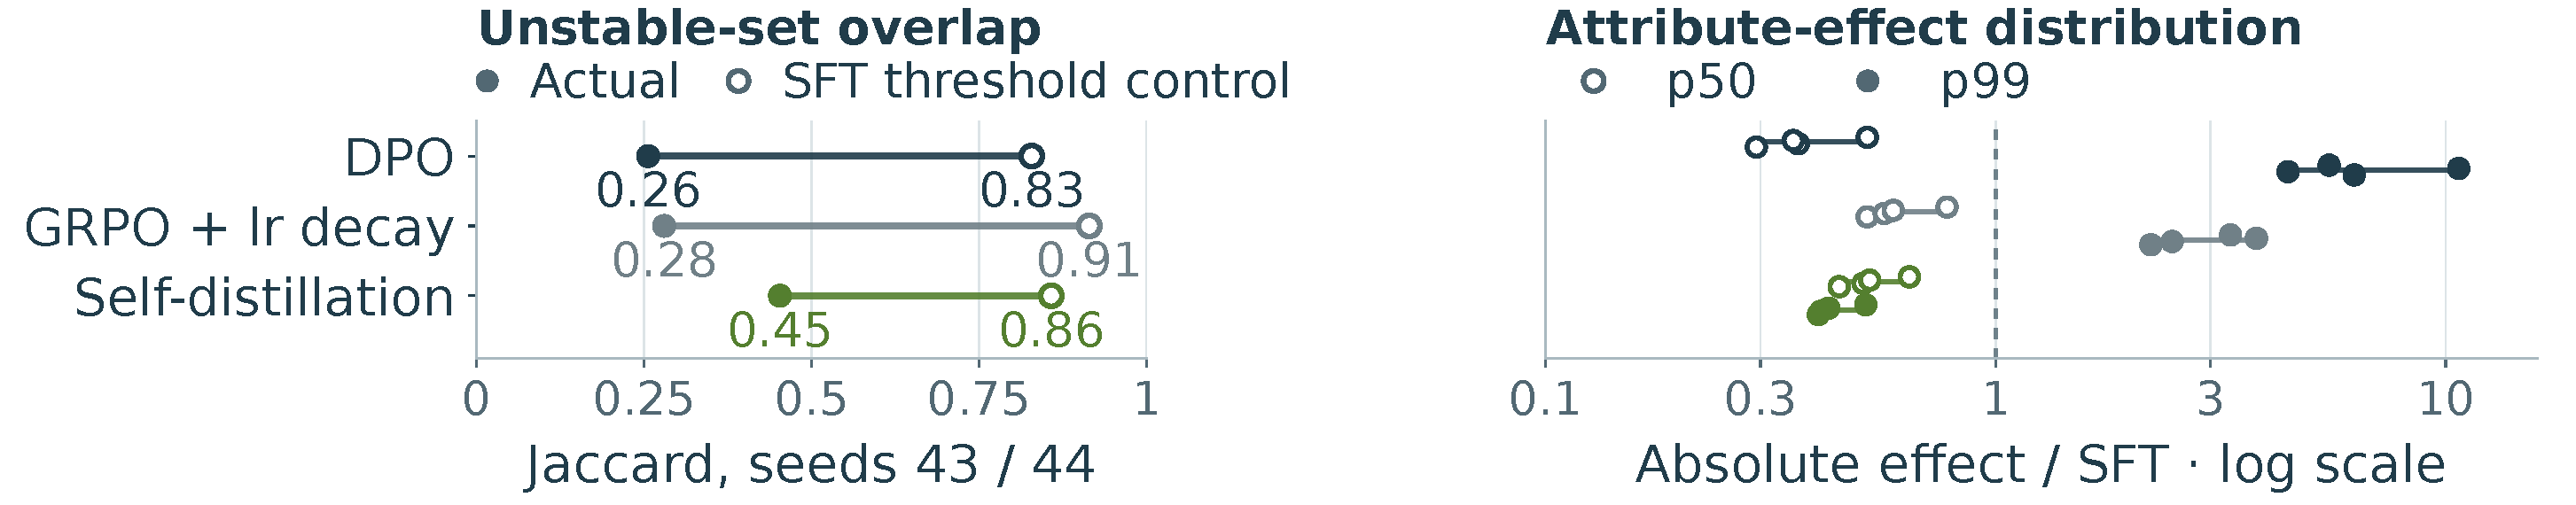
\includegraphics[width=16.666667in,keepaspectratio]{figures/residual.pdf}};
\Txt[text=muted]{488}{768}{768}{10.7}{Left: seeds 43/44 at each model's own threshold; control applies those thresholds to SFT-v3. Right: p50/p99 of absolute attribute effects relative to SFT-v3, all 450 pairs in four contrasts, one checkpoint per stage.}
\Rect{488}{809}{768}{45}{greenPale}
\Txt[text=ink]{498}{816}{748}{12.7}{\bfseries \BorderDistill{} of self-distillation's unstable sets come from \NBorder{} borderline pairs.}
\Txt[text=muted]{498}{835}{748}{10.7}{Own thresholds; \NBorder{} of \NPairs{} CV--job pairs have an SFT margin below 2. Sets within a pair share its CV and job.}
\Txt[text=muted]{488}{864}{768}{10.7}{Common-rate Jaccard over all seed pairs: DPO 0.17--0.28; GRPO 0.30--0.35; distillation 0.53--0.54. Same-cut SFT control: 1.00.}

% -------------------------- 4. MARTA'S ACTIVATION PATCHING --------------------
% Preserve Marta's original A/B drawing, terminology, bar data and core claims.
% Translation only: the original 700-unit content moves into the wider right panel.
\Rect{1296}{185}{720}{690}{panel}
\Section{1296}{185}{720}{24}{4. Methods and mechanistic findings}
\begin{scope}[shift={(800,-42)}]
\Txt[text=greenDark]{512}{284}{700}{16}{\bfseries A\quad HOW ACTIVATION PATCHING PROBES ATTRIBUTE EFFECTS}

% A1: copy one layer's activation from the attribute-B run into the attribute-A run.
\Txt[text=ink]{512}{314}{190}{13.5}{\bfseries Swap one activation}
\NodeBox{522}{338}{70}{22}{ink}{white}{10}{Attribute A}
\NodeBox{622}{338}{70}{22}{ink}{white}{10}{Attribute B}
\foreach \k in {0,...,4}{%
  \pgfmathsetmacro{\yy}{370+18*\k}
  \ifnum\k=2 \def\BarColour{ink}\else\def\BarColour{rule}\fi
  \Rect{527}{\yy}{60}{12}{\BarColour}
  \Rect{627}{\yy}{60}{12}{\BarColour}}
\draw[ink,line width=2.8bp,-{Latex[length=8bp,width=5.5bp]}] (627,412) to[bend right=55] (587,412);
\Txt[text=ink,align=center]{587}{384}{40}{11}{\bfseries swap}
% Result: how much of the attribute's effect disappears.
\Arrow{557}{458}{557}{470}
\Rect{522}{472}{170}{14}{rule}
\Rect{522}{472}{120}{14}{ink}
\Txt[text=body]{522}{491}{180}{10}{share of the attribute's effect removed}

% A2: the pathway. x = 770 + 11.2 * layer, so boxes sit over the layers they occupy.
\Txt[text=ink]{772}{314}{420}{13.5}{\bfseries Attribute-sensitive components in the Base model}
\Rect{998}{334}{56}{146}{rule}
\Txt[text=ink,align=center]{988}{337}{76}{10.5}{\bfseries bottleneck}
\NodeBox{772}{360}{68}{44}{ink}{white}{12.5}{Attribute}
\NodeBox{908}{360}{79}{44}{body}{white}{12}{Readers\\L7--14}
\NodeBox{993}{354}{66}{56}{ink}{mist}{13.5}{Hub\\L15.H11}
\draw[ink,line width=2.8bp] (993,354) rectangle ++(66,56);
\NodeBox{1116}{360}{66}{44}{body}{white}{12}{Readout\\MLP 31}
\NodeBox{1112}{420}{80}{22}{ink}{white}{11.5}{hire / reject}
% The main path, dashed: the boxes are patched components; the edges between them are not
% validated (no edge-level test), as the note beside B says.
\foreach \xa/\ya/\xb/\yb in {840/382/908/382,987/382/993/382,1059/382/1116/382,1149/404/1149/420}{%
  \draw[ink,dashed,line width=2.8bp,-{Latex[length=9bp,width=6.5bp]}] (\xa,\ya) -- (\xb,\yb);}
% Opposing heads push back on the signal between hub and readout.
\NodeBox{978}{440}{96}{24}{body}{white}{11.5}{Opposers}
\draw[gray,dashed,line width=2.3bp,-{Bar[width=9bp]}] (1074,452) -- (1090,452) -- (1090,385);
% Layer axis.
\draw[gray,line width=1.2bp] (830,486) -- (1177,486);
\foreach \L in {0,7,15,20,31}{%
  \pgfmathsetmacro{\xx}{830+11.2*\L}
  \draw[gray,line width=1.2bp] (\xx,482) -- (\xx,490);
  \Txt[text=body,align=center]{\xx-15}{494}{30}{11}{\L}}
\Txt[text=body]{772}{480}{50}{11}{layer}
% The diagram's labels by what patching them does (docs/INTERP_SFT_V3.md; the report's
% fig:circuit and its table of opposing heads, negative share).
\Txt[text=body]{512}{514}{700}{10.5}{\textbf{Readers}: layers 7--14 whose patch removes part of the effect upstream. \textbf{Hub}: the head whose patch removes the most. \textbf{Opposers}: heads whose patch increases the effect: they push against the bias. \textbf{Readout}: the last MLP, where the margin forms.}

% B: Base vs SFT-v3 on the same pairs. Left: attribute effect per pair; right: the hub head.
% Base gray, SFT-v3 ink, as in the results column.
\Rect[draw=greenDark,line width=1bp]{512}{546}{700}{102}{greenPale}
\Txt[text=greenDark]{526}{554}{500}{14}{\bfseries B\quad WHAT PATCHING FINDS: BASE VS SFT-v3, SAME PAIRS}
\Rect{1060}{558}{9}{9}{gray}\Txt[text=body]{1073}{556}{50}{11.5}{Base}
\Rect{1124}{558}{9}{9}{ink}\Txt[text=body]{1137}{556}{70}{11.5}{SFT-v3}
% Left: bars at 110 units per logit.
\foreach \r in {0,1,2,3}{%
  \pgfplotstablegetelem{\r}{label}\of\MechData\let\MLabel\pgfplotsretval
  \pgfplotstablegetelem{\r}{base}\of\MechData\let\MBase\pgfplotsretval
  \pgfplotstablegetelem{\r}{sft}\of\MechData\let\MSFT\pgfplotsretval
  \pgfplotstablegetelem{\r}{change}\of\MechData\let\MChange\pgfplotsretval
  \pgfmathsetmacro{\yy}{576+14*\r}
  \Txt[text=body]{526}{\yy}{94}{11}{\MLabel}
  \Rect{622}{\yy}{\MBase*110}{6}{gray}
  \Rect{622}{\yy+7}{\MSFT*110}{6}{ink}
  \Txt[text=ink]{\MBase*110+628}{\yy+1}{50}{11.5}{\bfseries\MChange}}
\Txt[text=body]{622}{634}{220}{10.5}{attribute effect per pair (logits)}
% Right: the same hub head carries far less; the claim is about patching effects, not a
% proven circuit (no edge-level test).
\Txt[text=ink]{928}{577}{284}{12}{\bfseries The hub head carries far less}
\draw[gray,line width=5bp] (928,604) -- (1168,604);
\draw[ink,line width=1.5bp] (928,617) -- (1168,617);
\NodeBox{1018}{596}{64}{30}{ink}{mist}{11.5}{L15.H11}
\draw[ink,line width=1.6bp] (1018,596) rectangle ++(64,30);
\Txt[text=gray]{1094}{589}{70}{11}{\bfseries\HubBase}
\Txt[text=ink]{1094}{620}{70}{11}{\bfseries\HubSFT}
\Txt[text=body]{928}{627}{240}{10.5}{logits / pair, combat implicit}
\end{scope}
% Selection and full-grid checks are outside the preserved A/B block.
\Txt[text=muted]{1312}{617}{688}{10.7}{\textbf{Same pairs within B}: Base and SFT-v3 use the same 64 pairs per contrast, selected on the Base effect. The diagram summarizes component interventions, not an edge-validated circuit.}
\Txt[text=muted]{1312}{652}{688}{10.7}{Across all 450 pairs, gender effect falls \GenderFullRemoval\% [\GenderFullRemovalCI\%, 95\% CI], versus 72\% in B's selected subset. The other three full-grid contrasts fall \OtherFullRemoval\%.}
\Txt[text=greenDark]{1312}{686}{688}{13.5}{\bfseries C\quad THE SAME TEST AFTER DPO, GRPO AND SELF-DISTILLATION}
\Txt[text=body]{1312}{707}{688}{10.7}{One checkpoint per stage. Pairs now selected on SFT-v3's own effect: 64 per contrast, gender 45. Real component-profile r vs SFT-v3:}
\Txt[text=ink]{1312}{739}{215}{12}{\bfseries DPO\quad \ProfDPO}
\Txt[text=ink]{1544}{739}{215}{12}{\bfseries GRPO\quad \ProfGRPO}
\Txt[text=ink]{1776}{739}{224}{12}{\bfseries Self-distillation\quad \ProfDistill}
\Txt[text=muted]{1312}{763}{688}{10.7}{Real head verification: DPO combat / implicit L23.H1 ranks first among \DPOLateTested{} tested heads, \DPOLateRealEffect{} logits per pair. Attribution patching selected candidate heads; this does not explain the tail cases.}
\Rect[draw=greenDark,line width=0.7bp]{1312}{802}{688}{66}{greenPale}
\Txt[text=greenDark]{1324}{810}{664}{13.3}{\bfseries Window-only LoRA did not match full layers}
\Txt{1324}{831}{490}{11.7}{Train only L15--20 / keep only its update / remove it}
\Txt[text=ink,align=right]{1826}{831}{162}{11.7}{\bfseries \WindowOnly{} / \WindowKept{} / \WindowRemoved{} pp}
\Txt[text=muted]{1324}{850}{664}{10.7}{Three-seed means, own rates. Capacity: \WindowParams{}M vs \StandardParams{}M parameters; rank-163 matched follow-up pending.}

% -------------------------- 5. NVIDIA COMPUTE --------------------------------
\Rect{48}{895}{1968}{138}{panel}
\Rect{48}{895}{1968}{31}{green}
\Txt[text=ink]{64}{900}{980}{22}{\bfseries 5. NVIDIA-accelerated audit}
\Txt[text=ink,align=right]{990}{907}{1010}{10.5}{CSCS Alps \quad GH200, 96 GB HBM3 \quad vLLM 0.31 \quad TRL / PEFT \quad PyTorch DDP, bf16}
\Txt[text=ink]{64}{934}{600}{12.2}{\bfseries Generation only: \AuditBenchPrompts{} prompts, \AuditBenchRepeats{} repeats}
\Txt{64}{955}{124}{12.0}{HF batch 8}
\Txt{64}{974}{124}{12.0}{HF batch 32}
\Txt{64}{993}{124}{12.0}{vLLM}
\Rect{190}{955}{290}{11}{gray}
\pgfmathsetmacro{\HFThirtyTwoWidth}{\AuditHFLargeSeconds/\AuditHFSmallSeconds*290}
\pgfmathsetmacro{\VLLMWidth}{\AuditVLLMSeconds/\AuditHFSmallSeconds*290}
\Rect{190}{974}{\HFThirtyTwoWidth}{11}{mist}
\Rect{190}{993}{\VLLMWidth}{11}{greenDark}
\Txt[text=ink]{491}{953}{170}{12.3}{\AuditHFSmallSeconds{} s}
\Txt[text=ink]{491}{972}{170}{12.3}{\AuditHFLargeSeconds{} s}
\Txt[text=ink]{491}{991}{170}{12.3}{\AuditVLLMSeconds{} s}
\Txt[text=muted]{64}{1012}{600}{10.4}{vLLM: \texttimes\AuditSpeedSmall{} vs HF8; \texttimes\AuditSpeedLarge{} vs HF32. Decision agreement \AuditBackendAgree\%.}
\draw[rule,line width=1bp] (674,936) -- (674,1021);
\Txt[text=ink]{692}{934}{328}{12.8}{\bfseries Full audit generation}
\Txt[text=greenDark]{692}{955}{328}{22}{\bfseries \AuditWallS{} s \quad \AuditKWh{} kWh}
\Txt{692}{985}{328}{12.3}{\FullAuditPrompts{} prompts; \FullAuditRepeats{} repeats\\\AuditReqPerS{} req/s during generation}
\Txt[text=muted]{692}{1015}{328}{10.4}{Wall time includes loading and writing; excludes scoring.}
\draw[rule,line width=1bp] (1036,936) -- (1036,1021);
\Txt[text=ink]{1054}{934}{475}{12.8}{\bfseries Training: 1 \textrightarrow{} 4 GH200 GPUs}
\ifnum\DDPReviewed=1
  \Txt[text=ink]{1054}{954}{475}{13.0}{\bfseries Training: \texttimes\DDPTrainingSpeedup{} wall speed; \DDPTrainingCostDelta\% GPU-h}
  \Txt[text=muted]{1054}{971}{475}{10.7}{Optimizer steps only.}
  \Txt[text=ink]{1054}{987}{475}{13.0}{\bfseries Whole step: \texttimes\DDPEndToEndSpeedup{} wall speed; \DDPCostDelta\% GPU-h}
  \Txt[text=muted]{1054}{1004}{475}{10.7}{Includes start-up, model merge and data preparation.}
  \Txt[text=muted]{1054}{1019}{475}{10.0}{Global batch \DDPBatch{}, \DDPSteps{} steps; GPU-h = elapsed time \texttimes{} used GPUs.}
\else
  \Txt{1054}{958}{475}{12.5}{Single-GPU repeat pending review.\\Report wall speed and used GPU-hours together.}
  \Txt[text=muted]{1054}{1008}{475}{9.4}{Same global batch \DDPBatch{}, \DDPSteps{} steps; both timing bases will be shown.}
\fi
\draw[rule,line width=1bp] (1536,936) -- (1536,1021);
\Txt[text=ink]{1554}{934}{446}{12.8}{\bfseries Mechanistic audit: one GH200}
\Txt{1554}{957}{446}{12}{64-pair patching: \PatchStepMin{} min, \PatchPeakGiB{} GiB peak}
\Txt{1554}{979}{446}{12}{Full margin scoring: \MarginsStepMin{} min, \MarginsPeakGiB{} GiB peak}
\Txt[text=muted]{1554}{1001}{446}{10.7}{Patching median, N=\PatchRunsSixtyFour{}; \PatchStepGPUh{} used GPU-h per run.\\Project: \ProjectGPUh{} allocated GPU-h; \ProjectKWh{} kWh logged by NVML.}

% -------------------------- TAKE-HOME / LIMITATION ---------------------------
\draw[greenDark,line width=1bp] (48,1040) -- (2016,1040);
\Txt[text=ink]{48}{1045}{1840}{14.2}{\bfseries SFT delivers the main gain. Additional training depends on the operating point and changes residual risk.}
\Txt[text=body]{48}{1067}{972}{10.8}{Three seeds matter: one DPO seed alone would have read as a 1 pp gain.}
\Txt[text=muted]{1038}{1067}{854}{10.8}{Limits: development benchmark; one selected checkpoint per mechanistic probe.}
\Txt[text=muted]{48}{1082}{1840}{9.4}{%
  \href{https://arxiv.org/abs/2106.09685}{[1] Hu et al., LoRA (2021)}\quad
  \href{https://arxiv.org/abs/2305.18290}{[2] Rafailov et al., DPO (2023)}\quad
  \href{https://arxiv.org/abs/2402.03300}{[3] Shao et al., GRPO (2024)}\quad
  \href{https://arxiv.org/abs/2301.04213}{[4] Hase et al., Does localization inform editing? (2023)}\quad
  \href{https://arxiv.org/abs/2309.16042}{[5] Zhang \& Nanda, Activation patching (2024)}\quad
  \href{https://github.com/Stereotypes-in-LLMs/hiring_bias_mitigation_at}{Code: github.com/Stereotypes-in-LLMs/hiring\_bias\_mitigation\_at}\quad
  \href{https://huggingface.co/datasets/Stereotypes-in-LLMs/hiring-bias-mitigation-v3}{Data: huggingface.co/datasets/Stereotypes-in-LLMs/hiring-bias-mitigation-v3}}
\node[anchor=north west,inner sep=0pt] at (1945,1047)
  {\qrcode[height=0.93in]{https://github.com/Stereotypes-in-LLMs/hiring\_bias\_mitigation\_at/blob/main/poster/DETAILS.md}};
\Txt[text=greenDark,align=right]{1894}{1092}{121}{9.4}{Results + code}

\end{scope}
\end{tikzpicture}
\end{document}
